\documentclass[tikz,border=8pt]{standalone}
\usepackage{tikz}
\usetikzlibrary{shapes.geometric,arrows.meta,positioning,calc,decorations.pathmorphing}
\usepackage{amsmath,amssymb}

\definecolor{mainblue}{RGB}{25,70,140}
\definecolor{accentred}{RGB}{180,50,30}
\definecolor{darkgreen}{RGB}{30,100,50}
\definecolor{darkgray}{RGB}{60,60,70}
\definecolor{gold}{RGB}{200,164,0}
\definecolor{purple}{RGB}{106,30,140}
\definecolor{teal}{RGB}{14,107,107}
\definecolor{lightblue}{RGB}{220,235,255}
\definecolor{lightgreen}{RGB}{220,245,220}
\definecolor{lightred}{RGB}{255,230,225}

% ─── Tikz-Stile ────────────────────────────────────────────────────────────
\tikzset{
  sysbox/.style={rectangle, rounded corners=4pt, draw=gray!70, fill=gray!8,
    minimum width=3.2cm, minimum height=1.1cm, align=center,
    font=\small\bfseries, text=black},
  arrow/.style={-{Stealth[length=6pt]}, thick, color=darkgray},
  doublearrow/.style={{Stealth[length=5pt]}-{Stealth[length=5pt]},
    thick, color=darkgray},
  layer/.style={rectangle, rounded corners=3pt, draw=gray!50, fill=gray!5,
    minimum width=13cm, minimum height=0.95cm, align=center,
    font=\small\bfseries, text=black},
  dnabase/.style={circle, draw=#1!80, fill=#1!20, minimum size=0.75cm,
    font=\bfseries\small, text=black},
}

% ═══════════════════════════════════════════════════════════════════════════
% TIKZ 1  –  DSS Schichtenmodell
% ═══════════════════════════════════════════════════════════════════════════
\begin{document}

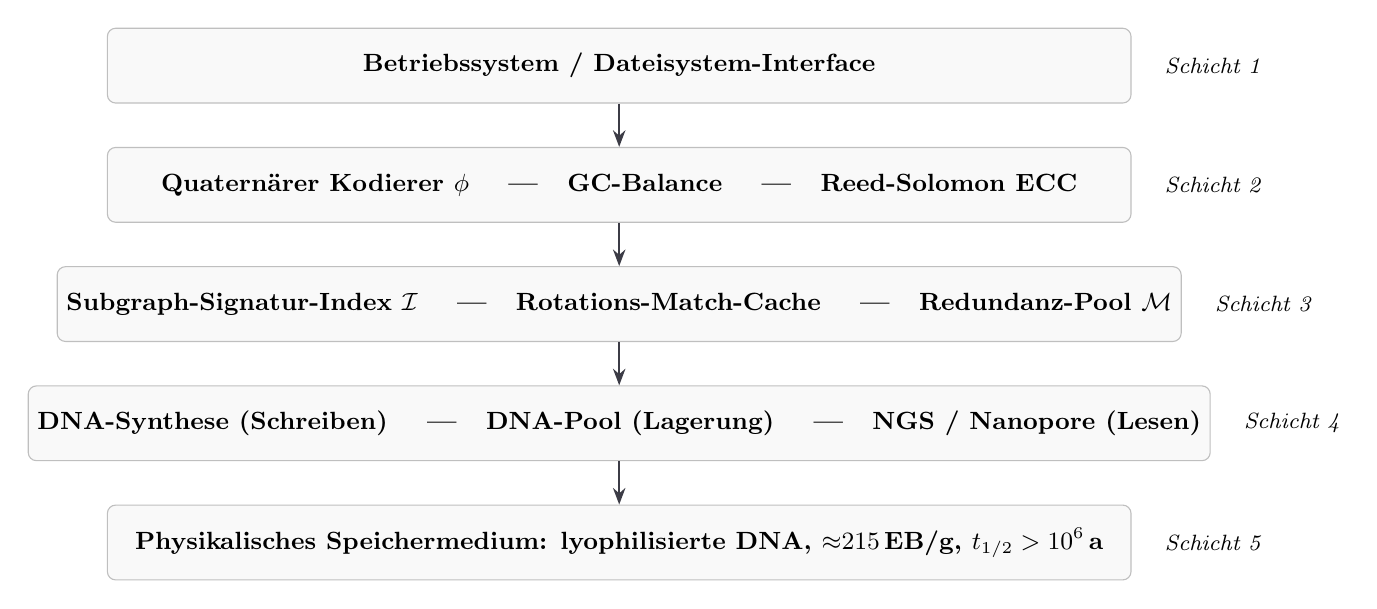
\begin{tikzpicture}[node distance=0.55cm]
  \node[layer=darkgray] (os)   {Betriebssystem / Dateisystem-Interface};
  \node[layer=mainblue, below=of os]  (cod)
        {Quaternärer Kodierer $\phi$ \quad|\quad GC-Balance \quad|\quad Reed-Solomon ECC};
  \node[layer=darkgreen, below=of cod] (idx)
        {Subgraph-Signatur-Index $\mathcal{I}$ \quad|\quad Rotations-Match-Cache \quad|\quad
         Redundanz-Pool $\mathcal{M}$};
  \node[layer=accentred, below=of idx] (hw)
        {DNA-Synthese (Schreiben) \quad|\quad DNA-Pool (Lagerung) \quad|\quad NGS / Nanopore (Lesen)};
  \node[layer=darkgray!70, below=of hw] (phy)
        {Physikalisches Speichermedium: lyophilisierte DNA, ${\approx}215\,\text{EB/g}$,
         $t_{1/2} > 10^6\,\text{a}$};

  \foreach \a/\b in {os/cod, cod/idx, idx/hw, hw/phy}
    \draw[arrow] (\a.south) -- (\b.north);

  % Beschriftungen
  \node[font=\footnotesize\itshape, right=0.3cm of os]  {Schicht 1};
  \node[font=\footnotesize\itshape, right=0.3cm of cod] {Schicht 2};
  \node[font=\footnotesize\itshape, right=0.3cm of idx] {Schicht 3};
  \node[font=\footnotesize\itshape, right=0.3cm of hw]  {Schicht 4};
  \node[font=\footnotesize\itshape, right=0.3cm of phy] {Schicht 5};
\end{tikzpicture}

\newpage

% ═══════════════════════════════════════════════════════════════════════════
% TIKZ 2  –  Quaternäres Kodierungsschema (Bijektion)
% ═══════════════════════════════════════════════════════════════════════════
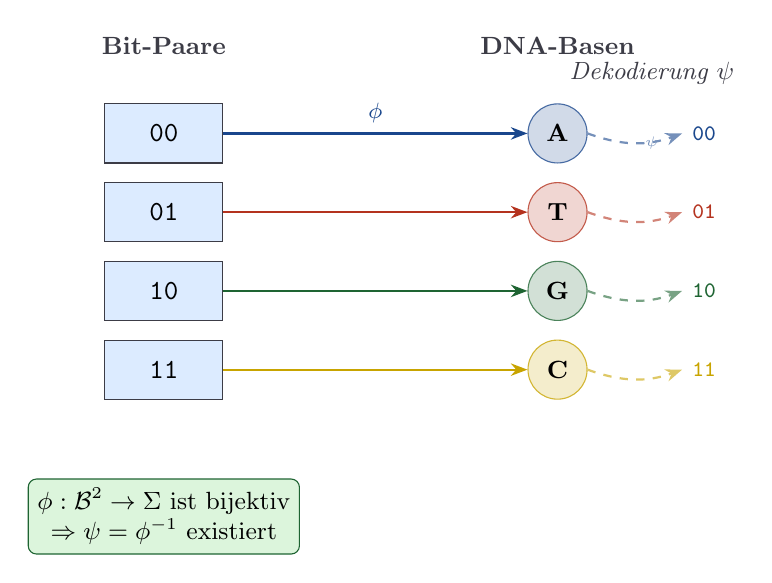
\begin{tikzpicture}[node distance=1.2cm and 2.5cm]
  % Bit-Paare
  \foreach \bits/\y in {00/3, 01/2, 10/1, 11/0}{
    \node[rectangle, draw=darkgray, fill=lightblue, minimum width=1.5cm,
          minimum height=0.75cm, font=\bfseries] (b\bits) at (0,\y)
          {\texttt{\bits}};
  }
  % Basen
  \node[dnabase=mainblue]  (A) at (5,3) {A};
  \node[dnabase=accentred] (T) at (5,2) {T};
  \node[dnabase=darkgreen] (G) at (5,1) {G};
  \node[dnabase=gold]      (C) at (5,0) {C};

  % Bijektionspfeile
  \draw[arrow, mainblue]  (b00.east) -- node[above,font=\footnotesize]{$\phi$} (A.west);
  \draw[arrow, accentred] (b01.east) -- (T.west);
  \draw[arrow, darkgreen] (b10.east) -- (G.west);
  \draw[arrow, gold]      (b11.east) -- (C.west);

  % Rückwärtspfeile (Dekodierung)
  \draw[arrow, mainblue!60,  dashed] (A.east) to[bend right=20]
        node[right,font=\tiny]{$\psi$} ++(1.2,0)
        node[right,font=\footnotesize,mainblue]{\texttt{00}};
  \draw[arrow, accentred!60, dashed] (T.east) to[bend right=20]
        ++(1.2,0) node[right,font=\footnotesize,accentred]{\texttt{01}};
  \draw[arrow, darkgreen!60, dashed] (G.east) to[bend right=20]
        ++(1.2,0) node[right,font=\footnotesize,darkgreen]{\texttt{10}};
  \draw[arrow, gold!60,      dashed] (C.east) to[bend right=20]
        ++(1.2,0) node[right,font=\footnotesize,gold]{\texttt{11}};

  % Labels
  \node[above=0.5cm of b00, font=\bfseries\small, darkgray] {Bit-Paare};
  \node[above=0.5cm of A,   font=\bfseries\small, darkgray] {DNA-Basen};
  \node[above=0.5cm of A -| {(6.2,3)}, font=\small\itshape, darkgray]
        {Dekodierung~$\psi$};

  % Bijektivitätsannotation
  \node[draw=darkgreen, fill=lightgreen, rounded corners=3pt,
        font=\small, align=center, below=1.0cm of b11]
        {$\phi: \mathcal{B}^2 \to \Sigma$ ist bijektiv\\
         $\Rightarrow \psi = \phi^{-1}$ existiert};
\end{tikzpicture}

\newpage

% ═══════════════════════════════════════════════════════════════════════════
% TIKZ 3  –  Subgraph-Signatur-Index (Retrieval-Struktur)
% ═══════════════════════════════════════════════════════════════════════════
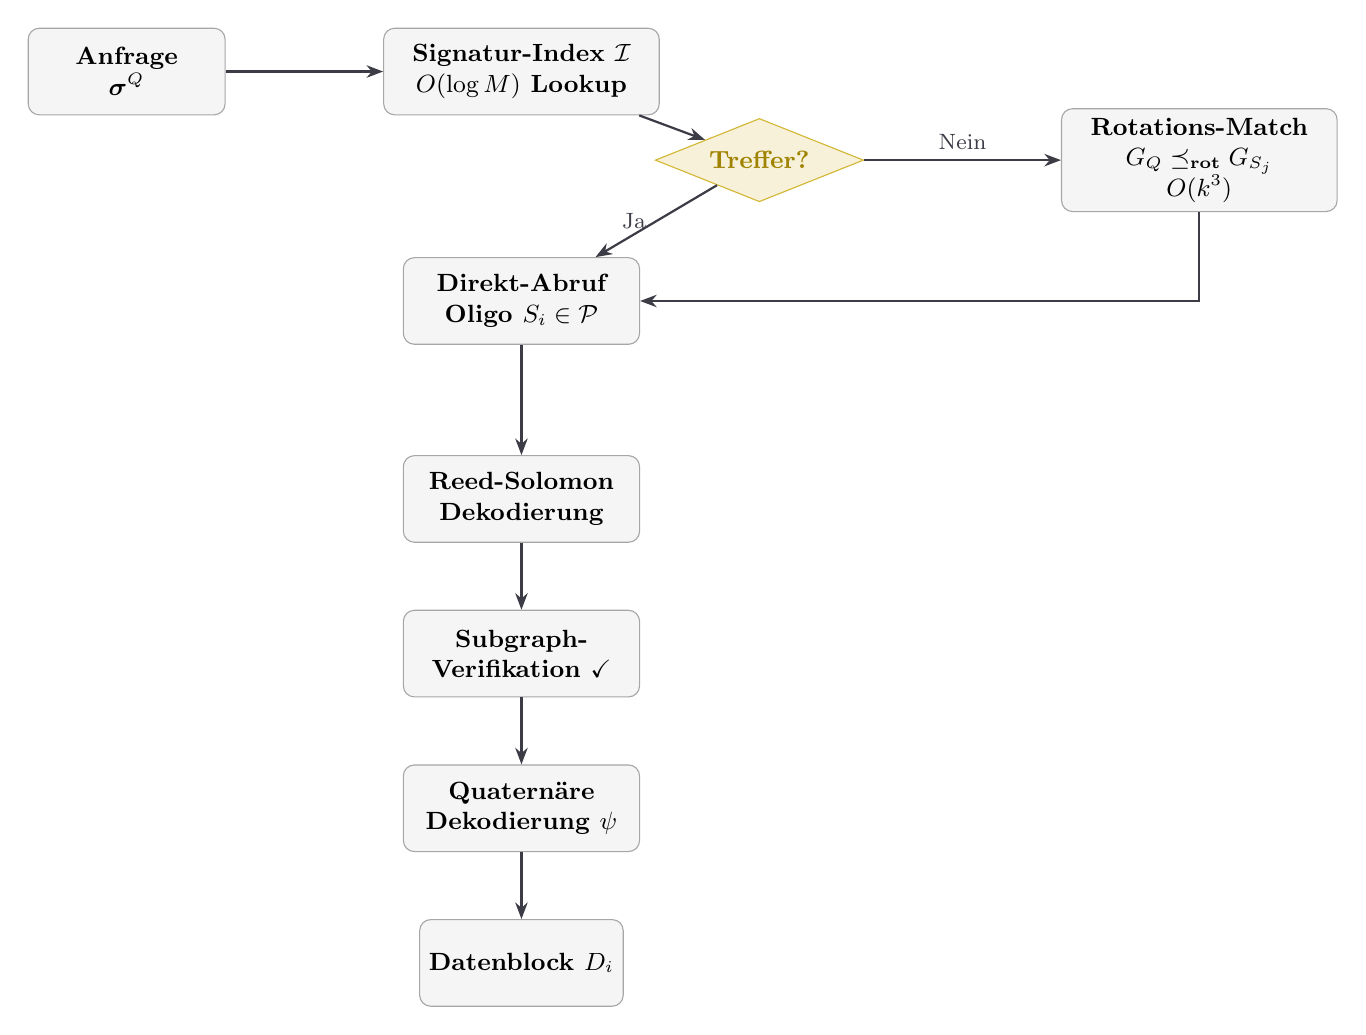
\begin{tikzpicture}[node distance=0.9cm and 1.8cm]
  % Query
  \node[sysbox=mainblue, minimum width=2.5cm] (query) at (0,0)
        {Anfrage\\$\boldsymbol{\sigma}^Q$};

  % Hash-Index
  \node[sysbox=teal, right=2.0cm of query, minimum width=3.5cm] (index)
        {Signatur-Index $\mathcal{I}$\\$O(\log M)$ Lookup};

  % Cache-Entscheidung
  \node[diamond, draw=gold!80, fill=gold!15, aspect=2.5,
        below right=0.3cm and 0.6cm of index, font=\small\bfseries,
        text=gold!80!black] (hit) {Treffer?};

  % Cache-Hit-Pfad
  \node[sysbox=darkgreen, below=1.8cm of index, minimum width=3.0cm]
        (direct) {Direkt-Abruf\\Oligo $S_i \in \mathcal{P}$};

  % Cache-Miss-Pfad
  \node[sysbox=accentred, right=2.5cm of hit, minimum width=3.5cm]
        (rotmatch) {Rotations-Match\\$G_Q \preceq_\text{rot} G_{S_j}$\\$O(k^3)$};

  % ECC + Verify
  \node[sysbox=purple, below=1.4cm of direct, minimum width=3.0cm]
        (ecc) {Reed-Solomon\\Dekodierung};
  \node[sysbox=darkgray, below=0.85cm of ecc, minimum width=3.0cm]
        (verify) {Subgraph-\\Verifikation $\checkmark$};
  \node[sysbox=darkgreen, below=0.85cm of verify, minimum width=3.0cm]
        (decode) {Quaternäre\\Dekodierung $\psi$};
  \node[sysbox=mainblue, below=0.85cm of decode, minimum width=2.5cm]
        (out) {Datenblock $D_i$};

  % Pfeile
  \draw[arrow] (query) -- (index);
  \draw[arrow] (index) -- (hit);
  \draw[arrow] (hit)   -- node[left,font=\footnotesize]{Ja} (direct);
  \draw[arrow] (hit)   -- node[above,font=\footnotesize]{Nein} (rotmatch);
  \draw[arrow] (rotmatch) |- (direct);
  \draw[arrow] (direct) -- (ecc);
  \draw[arrow] (ecc)    -- (verify);
  \draw[arrow] (verify) -- (decode);
  \draw[arrow] (decode) -- (out);
\end{tikzpicture}

\newpage

% ═══════════════════════════════════════════════════════════════════════════
% TIKZ 4  –  DNA-Datengraph eines Datenblockes
% ═══════════════════════════════════════════════════════════════════════════
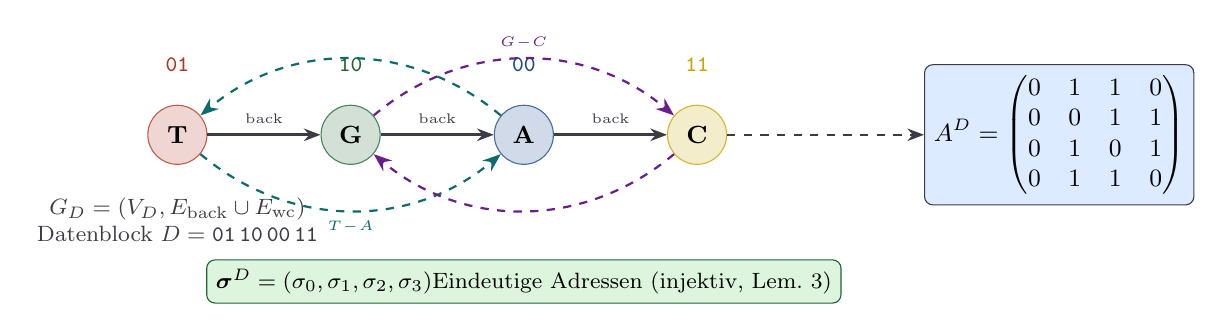
\begin{tikzpicture}[node distance=1.8cm]
  % Beispielsequenz  D = 01 10 00 11  →  S = T G A C
  \node[dnabase=accentred] (T) at (0,0)   {T};
  \node[dnabase=darkgreen] (G) at (2.2,0) {G};
  \node[dnabase=mainblue]  (A) at (4.4,0) {A};
  \node[dnabase=gold]      (C) at (6.6,0) {C};

  % Bit-Labels
  \node[above=0.3cm of T, font=\footnotesize, accentred]  {\texttt{01}};
  \node[above=0.3cm of G, font=\footnotesize, darkgreen] {\texttt{10}};
  \node[above=0.3cm of A, font=\footnotesize, mainblue]  {\texttt{00}};
  \node[above=0.3cm of C, font=\footnotesize, gold]      {\texttt{11}};

  % Backbone-Kanten
  \draw[arrow, darkgray, very thick] (T) -- node[above,font=\tiny]{back} (G);
  \draw[arrow, darkgray, very thick] (G) -- node[above,font=\tiny]{back} (A);
  \draw[arrow, darkgray, very thick] (A) -- node[above,font=\tiny]{back} (C);

  % Watson-Crick-Kanten (komplementär: T–A und G–C)
  \draw[-{Stealth}, teal, thick, dashed, bend right=40]
        (T) to node[below,font=\tiny,teal]{$T\!-\!A$} (A);
  \draw[-{Stealth}, teal, thick, dashed, bend right=40]
        (A) to (T);
  \draw[-{Stealth}, purple, thick, dashed, bend left=40]
        (G) to node[above,font=\tiny,purple]{$G\!-\!C$} (C);
  \draw[-{Stealth}, purple, thick, dashed, bend left=40]
        (C) to (G);

  % Adjazenzmatrix
  \node[draw=darkgray, fill=lightblue, rounded corners=3pt,
        font=\small, right=2.5cm of C, align=left] (mat)
  {$A^D = \begin{pmatrix}
      0&1&1&0\\0&0&1&1\\0&1&0&1\\0&1&1&0
   \end{pmatrix}$};
  \draw[arrow, darkgray, dashed] (C.east) -- (mat.west);

  % Signaturwerte
  \node[draw=darkgreen, fill=lightgreen, rounded corners=3pt,
        font=\footnotesize, below=1.2cm of A] (sig)
        {$\boldsymbol{\sigma}^D = (\sigma_0, \sigma_1, \sigma_2, \sigma_3)$\\
         Eindeutige Adressen (injektiv, Lem.~3)};

  \node[below=0.3cm of T, font=\footnotesize, darkgray, align=center]
        {$G_D = (V_D, E_{\text{back}} \cup E_{\text{wc}})$\\
         Datenblock $D = \texttt{01\,10\,00\,11}$};
\end{tikzpicture}

\newpage

% ═══════════════════════════════════════════════════════════════════════════
% TIKZ 5  –  Subgraph-Komprimierung: Inklusionsbaum
% ═══════════════════════════════════════════════════════════════════════════
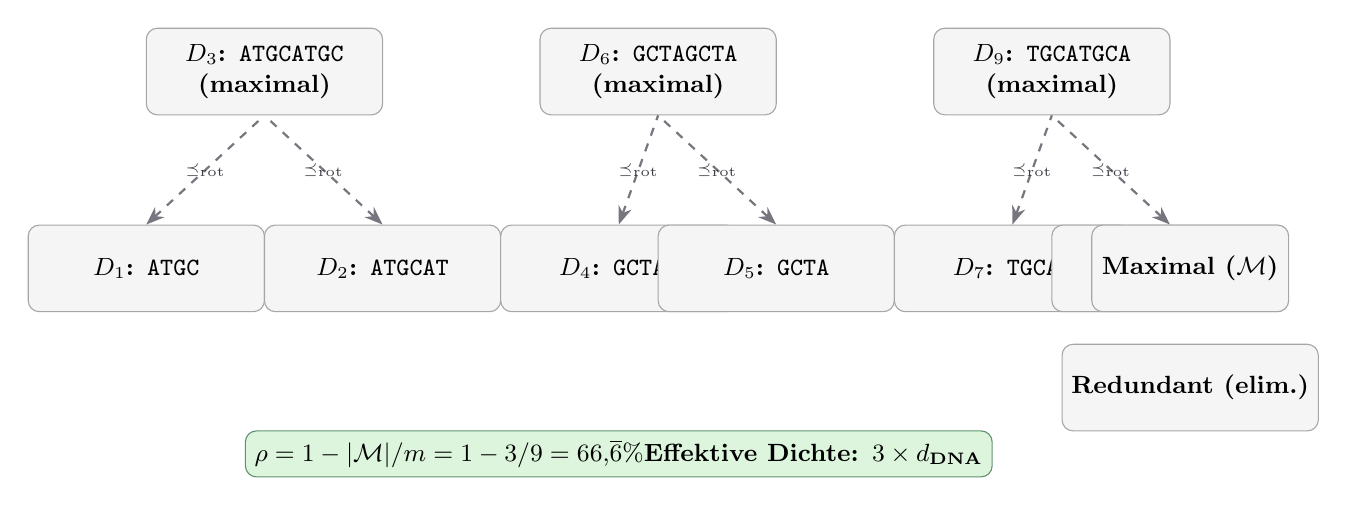
\begin{tikzpicture}[node distance=1.1cm and 2.5cm,
  maxnode/.style={sysbox=darkgreen, minimum width=3.0cm},
  rednode/.style={sysbox=accentred, minimum width=3.0cm}]

  % Maximale Knoten (Kerngenom)
  \node[maxnode] (M1) at (0, 0)    {$D_3$: \texttt{ATGCATGC}\\(maximal)};
  \node[maxnode] (M2) at (5, 0)    {$D_6$: \texttt{GCTAGCTA}\\(maximal)};
  \node[maxnode] (M3) at (10, 0)   {$D_9$: \texttt{TGCATGCA}\\(maximal)};

  % Redundante Knoten
  \node[rednode] (R1) at (-1.5,-2.5) {$D_1$: \texttt{ATGC}};
  \node[rednode] (R2) at (1.5, -2.5) {$D_2$: \texttt{ATGCAT}};
  \node[rednode] (R3) at (4.5, -2.5) {$D_4$: \texttt{GCTAG}};
  \node[rednode] (R4) at (6.5, -2.5) {$D_5$: \texttt{GCTA}};
  \node[rednode] (R5) at (9.5, -2.5) {$D_7$: \texttt{TGCAT}};
  \node[rednode] (R6) at (11.5,-2.5) {$D_8$: \texttt{TGC}};

  % Subgraph-Inklusionspfeile (rot → max)
  \foreach \r/\m in {R1/M1, R2/M1, R3/M2, R4/M2, R5/M3, R6/M3}
    \draw[{Stealth}-,thick,darkgray!70,dashed] (\r.north) --
          node[midway,font=\tiny,darkgray]{$\preceq_\text{rot}$} (\m.south);

  % Legende
  \node[maxnode, right=0.5cm of M3 |- R1, minimum width=2.5cm] (leg1)
        {Maximal ($\mathcal{M}$)};
  \node[rednode, below=0.4cm of leg1, minimum width=2.5cm] (leg2)
        {Redundant (elim.)};

  % Komprimierungsrate
  \node[draw=darkgreen!70, fill=lightgreen, rounded corners=4pt,
        font=\small\bfseries, below=1.5cm of R3] (cr)
        {$\rho = 1 - |\mathcal{M}|/m = 1 - 3/9 = 66{,}\overline{6}\%$\\
         Effektive Dichte: $3\times d_{\text{DNA}}$};
\end{tikzpicture}

\end{document}
